\section{Large pictures}

\begin{figure}[h]
    \centering
     \begin{subfigure}[h]{.65\textwidth}
         \centering
         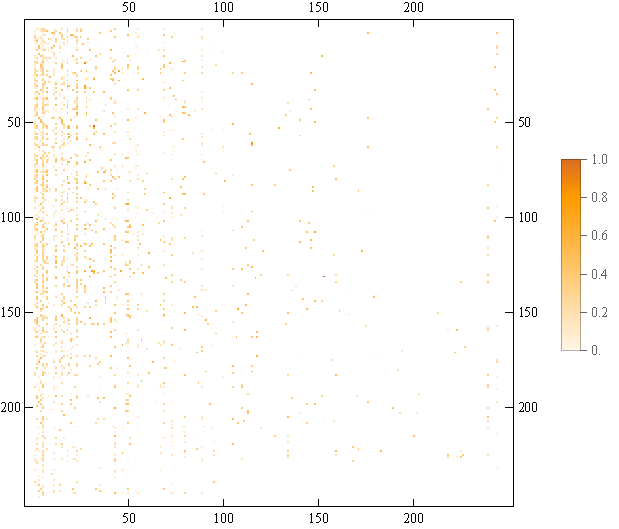
\includegraphics[width=\textwidth]{assets/asymmPlotFull.pdf}
         \caption{Original rate matrix}
         \label{fig:asymm-plot-full}
     \end{subfigure}
     \hfill
     \begin{subfigure}[h]{.65\textwidth}
         \centering
         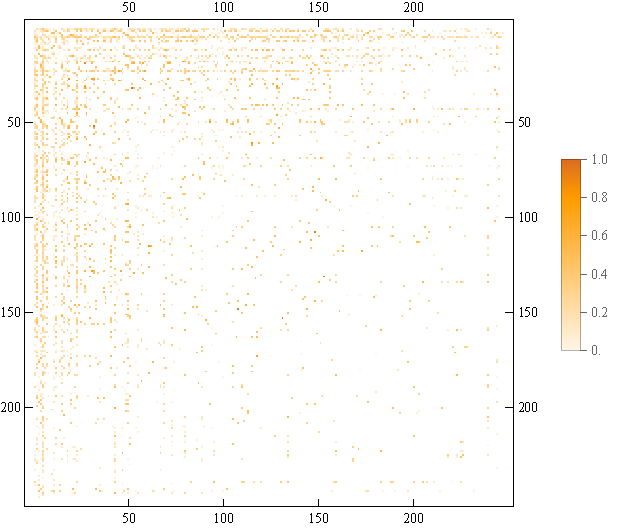
\includegraphics[width=\textwidth]{assets/symmPlotFull.pdf}
         \caption{Symmetrized rate matrix}
         \label{fig:symm-plot}
     \end{subfigure}
     \caption{Plot of the full, normalized rate matrix, sorted by city population.}
\end{figure}

\begin{figure}[b]
    \centering
    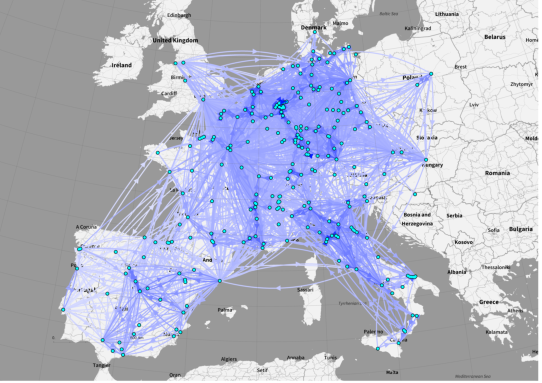
\includegraphics[angle=-90,origin=c,width=1\linewidth]{report/assets/rasterBigPlot.pdf}
    \caption{Big plot of the whole (unsymmetrized) network. The color of each arrow is proportional to its respective weight in the rate matrix $W$.}
    \label{fig:big-plot}
\end{figure}
